\documentclass[a4paper,10pt,twocolumn]{article}
\usepackage{lmodern}
%\usepackage[czech]{babel}
\usepackage[T1]{fontenc}
\usepackage[utf8]{inputenc}
\usepackage{graphicx}
\usepackage{float}
\usepackage[top=0.5cm,bottom=2cm,left=1cm,right=1cm]{geometry}
\usepackage{booktabs}
\usepackage{hyperref}
\hypersetup{
     colorlinks=true, % Otherwise the links are in color boxes.
     linkcolor=black, % E.g. hyperlinks in table of contents.
     citecolor=black,
     urlcolor=blue, % Classical blue web links.
     }


\title{Technical Report of NI-ROZ Term Project \\ WLD: A Robust Local Image Descriptor}
\date{\today}
\author{Jaroslav Langer \\ langeja5@cvut.cz}


\begin{document}
\maketitle

\begin{abstract}
Weber Local Descriptor (WLD) was shown to be a powerful technique for texture classification and face detection.
In this work I evaluated its performance on classification of skin lesions.
Based on these experiments the WLD does not seem to be the right tool for this job.
First probable reason for WLD's poor performance is the low-contrast nature of these pictures.
Second likely reason is the inherent imbalance of the dataset i.e. dominance of the benign samples.
\end{abstract}


\section{Introduction}
Classification of skin lesion images is a multi step process.
Following section describes in detail the implementation of Weber Local Descriptor\cite{chen2010wld}.
WLD is a feature extraction method inspired by Weber's Law from psychology, hence the name.
For a given image it produces features called WLD histogram.
Later section of this work describes how these histograms were used to classify the skin lesions.


\section{Weber Local Descriptor}
% 
In a broader sense, WLD is a local dense descriptor which extracts features pixel by pixel over the input image.
Local it's because it encodes the image piece by piece.
It does not try to capture the global information at once.
The word dense means it encodes all the local regions, it does not select between them.
It is composed of two parts.
The first part is about pixel's differential excitation in contrast to its neighbors.
Second part of WLD is a pixel gradient orientation known from the HoG technique.
Combination of these parts produces the WLD histogram.

\subsection{Differential Excitation}

Weber's law basically says, threshold for noticeable stimulus change is a multiple of the stimulus original intensity.
This can be phrased in multiple ways, however following quotation illustrates it the best.
"So, for example, in a noisy environment one must shout to be heard while a whisper works in a quiet room."\cite{chen2010wld}.
The differential excitation is inspired by this law.
For one pixel it is calculated as intensity difference of neighbor pixels to it's value divided by the value.
Let $x_i \quad i = 0, 1, \dots p-1$ denote the neighbors of $x_c$, then equation for differential excitation $\xi(x_c)$ is of form:
$$\xi(x_c) = \textrm{arctan} \left ( \sum_{i=0}^{p-1}{\frac{x_i-x_c}{x_c}} \right )$$
A hope for this approach is to extract the same features that stimulate the human perception.
That is why authors \cite{chen2010wld} say this component should extract the most important information.

\subsection{Gradient Orientation}

The gradient orientation is calculated using two convolution kernel filters and an atan2 function.
For a pixel its gradient orientation is calculated by atan2 given the 2D convolution of square pixel neighborhood with these two kernels $[-1,0,1]$ and $[-1,0,1]^{\top}$.
The gradient orientation $\theta(x_c)$ is in range $(-\pi, \pi)$.
Based on the original WLD implementation the values are binned into T bins and slightly rotated so the direction such as straight up or down are not on the edge but in the middle of the bin.

\begin{figure}[H]
       \begin{center}
              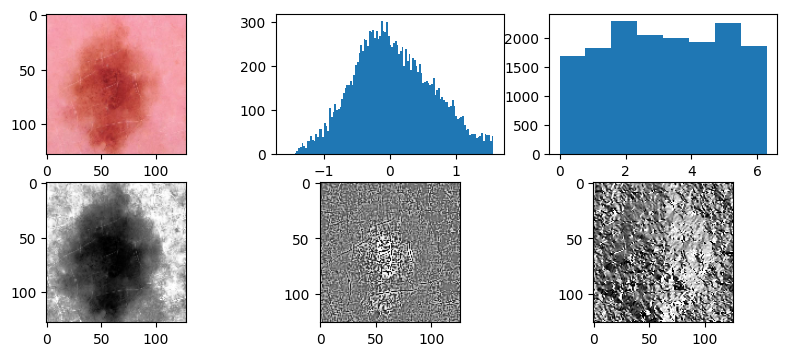
\includegraphics[width=6cm]{benign_overview}
              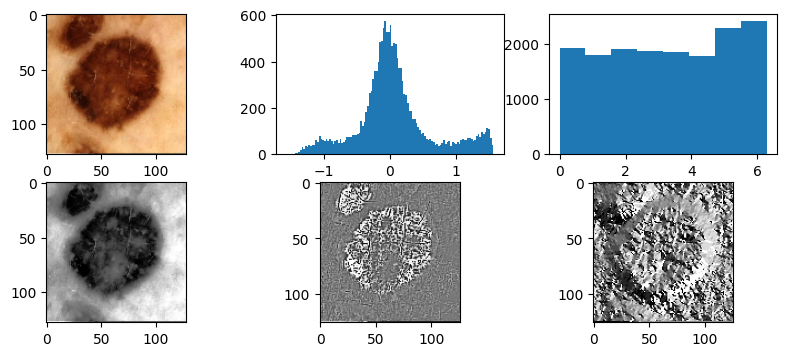
\includegraphics[width=6cm]{malignant_overview}
       \end{center}
       \caption{Visualizations of two typical correctly classified skin lesions, upper six is benign, lower six is malignant. In the first column there is the original cropped image and its histogram-equalized grayscale transformation. Differential excitation is in the middle column and on the right is the gradient orientation.}
       \label{fig1}
\end{figure}

\subsection{WLD Histogram}

Having calculated the differential excitation $\xi$ and gradient orientations $\theta$ we can construct WLD histogram.
The first step is to create a two dimensional histogram by binning $\xi$ into $M$ bins and $\theta$ into $T$ bins.
Then order these groups first by $\xi$ values.
Let's denote values belonging into first $\xi$ bin and first $\theta$ bin as $G_{\xi_0, \theta_0}$, then the WLD values are in following order:
$$WLD = G_{\xi_0, \theta_0}, G_{\xi_0, \theta_1},... $$
Now from each group $G$ made a histogram $H$ by binning its $\xi$ values into $T$ bins.
Last step is to concatenate these histograms in the order previously described.
Just to summarize how to WLD histogram looks.
It starts with $S$ differential excitation bins form the range of first $M$ bin and from first gradient orientation bin $T$.
Then there are another $S$ differential excitation bins still from the first $M$ bin range, but from the second gradient orientation bin $T$.
And this continues.
So the differential excitation extremes are on the both ends of the WLD histogram.
Last step is to normalize it, so the sum of WLD equals to 1.

\begin{figure}[H]
      \begin{center}
            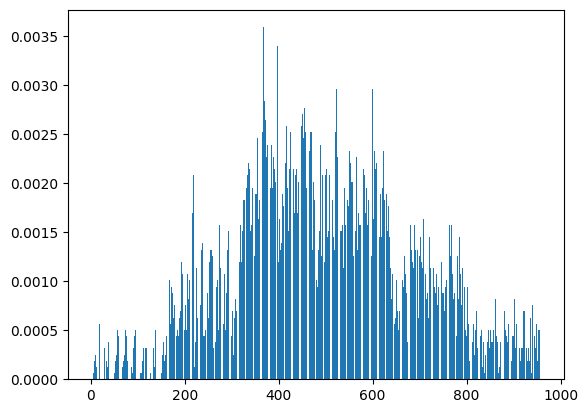
\includegraphics[width=4cm]{benign_wld}
            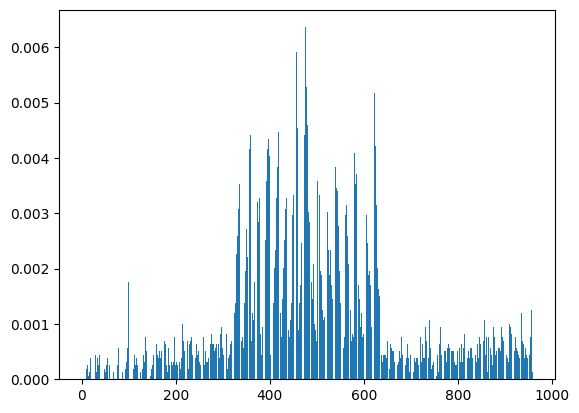
\includegraphics[width=4cm]{malignant_wld}
      \end{center}
      \caption{WLD histograms of images from Figure \ref{fig1}, the benign on the left, malignant on the right. It is visible the general structure of the histogram resembles the differential excitation.}
      \label{fig2}
\end{figure}


\section{Melanoma Detection}

The WLD was used to classify images\cite{isicarchiveISIC2020} to benign and malignant.
All evaluations were done solely on the "Train" images.
This is because the published dataset misses ground truth for the test images.
Nevertheless the Train data were always divided into train and test parts.
And no information from the test part was leveraged.
This division to train and test section was done multiple times, in order to eliminate potential split luck.

\subsection{Size and Scale}

As a first preprocessing step I cropped all images to the biggest possible center square.
In some cases it led to omitting small part of the skin lesion on a side.
After this I downscaled all the images in to 512x512 pixels.
In the original paper they report several image sizes.
However non of it was bigger than 200x200, so I considered this to be safe.
In contrast to the paper I didn't divide any image into parts.

\subsection{Color Channels and Distributions}

The original paper worked with already grayscale images and the color ones converted to grayscale.
I evaluated both conventional conversion to grayscale and calculating WLDs for every channel and ten concatenating the histograms.
In the original work they also applied histogram equalization of the images.
I evaluated both equalization both on grayscale and on per color channel.

\subsection{Histogram distance}

In the paper they report using intersection of normalized WLS histograms.
As this similarity is in the range of (0, 1), where 0 means disjoint histograms and 1 means identical.
It is easy to convert the similarity to distance. 
$$\textrm{dist}(a, b) = 1 - \sum_{i=1}^{bins} \min(h_{WLS}(a)_i, h_{WLS}(b)_i)$$


\subsection{Classifiers}

The classification was done using K-Nearest Neighbors and Support Vector Machine classifiers.
In the original paper, the KNN was used for texture classification whereas the VSM was used for a face detection.
I tested two KNN settings and that is One-Nearest Neighbor, and 3-Nearest Neighbors (3-NN).
For SVM I tested two kernels the polynomial of 3rd degree (poly(3)) and the radial basis function (rbf).
SVM with a polynomial kernel of second degree was also tested but underperformed the poly(3) significantly so its testing was not extensive.

\section{Results}

The results are admittedly rather poor.
No matter the parameters the balanced accuracy (i.e. arithmetic mean of true positive rate and true negative rate) was always between 0.49 and 0.54.
The same surprisingly holds when WLD histogram was created by concatenation of sub WLD histograms for each color channel.
And these accuracies were only for the One Nearest Neighbor classifier.
All the other classifiers 3NN, VSM-poly(3) and VSM-rbf were usually at 0.5 as there were not able to classify any melanoma.

There are probably two biggest factors of WLD low performance.
The first factor I will call low-contrast patterns.

The skin lesion dataset is very "flat" in comparison to both texture and face images from the paper.
The support for this claim is that the in the paper the authors say the differential excitation histogram has a U shape.
It means there are a lot of high excitation differences in either direction.
On the other hand, typical differential excitation histogram of the skin lesion image is sharp "hill".
It is possible to obtain the U shape by downscaling the image to 32x32 pixels (this size was used in the paper also).
The images starts to be more contrasting thanks to it, however the performance is then worse.

Second main issue is the imbalance of the classes.
In the original paper the textures were balanced and they had abundance of face samples.
The skin dataset is the opposite, the malignant samples are the absolute minority.

When I tested the WLD on balanced set of images I got balanced accuracy of 0.66.
It is remarkably better than 0.54, however it does not seem useful for an application.
When I balanced only the training set the balanced accuracies on the real test set were again 0.5 or even worse.

\section{Conclusion}

WLD is a understandable tool with published qualities on some tasks.
Even though it is quite a robust technique\cite{chen2010wld} it is definitely not suitable for all tasks.
One such a task the WLD is not sufficient is the classification of skin lesions at least based my experiments.
On the other hand, authors of the original paper used several techniques that could improve the performance significantly.
For the faces detection they had curated samples of clean faces.
I took the images as is, just cropped to the square shape.
They also build and ensemble of weak classifiers for segments of the image.
I used only one classifier.
And lastly they weighed the excitation intervals to improve the classification accuracy. 
I chose to not do it as there wouldn't be much data left for training and testing if all these things should be on different data.


\bibliographystyle{unsrt}
\bibliography{references}

\appendix

\section{Classification Examples}

\begin{figure}[H]
    \begin{center}
    \begin{tabular}{llrr}
    \toprule
    test\_size & name &   mean &  std \\
    \midrule
    0.3 & KNN-1 &  0.516579 &  0.018630 \\
        & KNN-3 &  0.508391 &  0.011541 \\
        & SVM-poly3 &  0.506888 &  0.007571 \\
        & SVM-rbf &  0.500000 &  0.000000 \\
    0.5 & KNN-1 &  0.519423 &  0.009837 \\
        & KNN-3 &  0.506480 &  0.005978 \\
        & SVM-poly3 &  0.504953 &  0.003884 \\
        & SVM-rbf &  0.500000 &  0.000000 \\
    0.7 & KNN-1 &  0.514081 &  0.006601 \\
        & KNN-3 &  0.502249 &  0.001457 \\
        & SVM-poly3 &  0.502845 &  0.003888 \\
        & SVM-rbf &  0.500000 &  0.000000 \\
    \bottomrule
    \end{tabular}
    \end{center}
    \caption{Bal. accuracy, paper settings no weights, side 128p.}
    \label{fig3}
\end{figure}


\begin{figure}[H]
      \begin{center}
            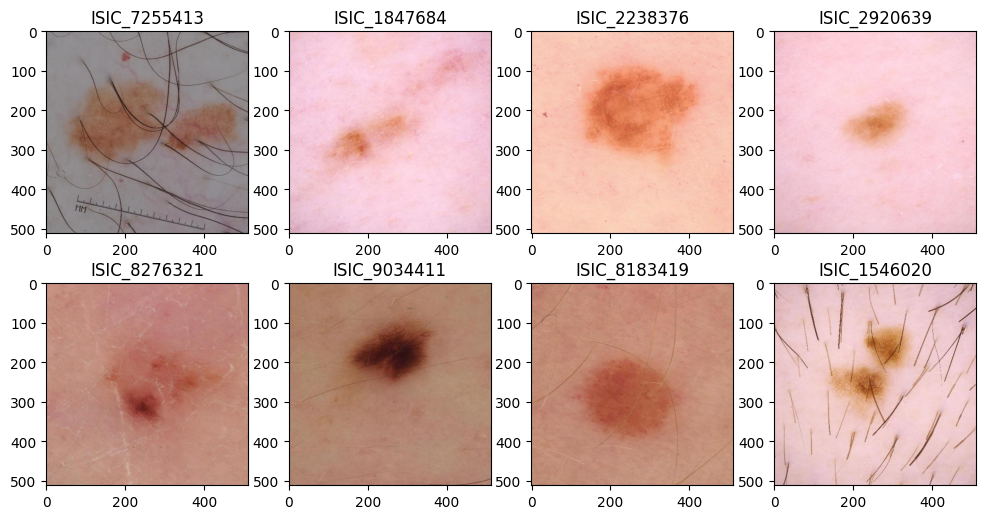
\includegraphics[width=8cm]{true_negative}
      \end{center}
      \caption{True negative examples. Usually images with little differential excitation, i.e. smooth hill with maximum in zero, see Figure \ref{fig1}.}
      \label{fig4}
\end{figure}

\begin{figure}[H]
      \begin{center}
            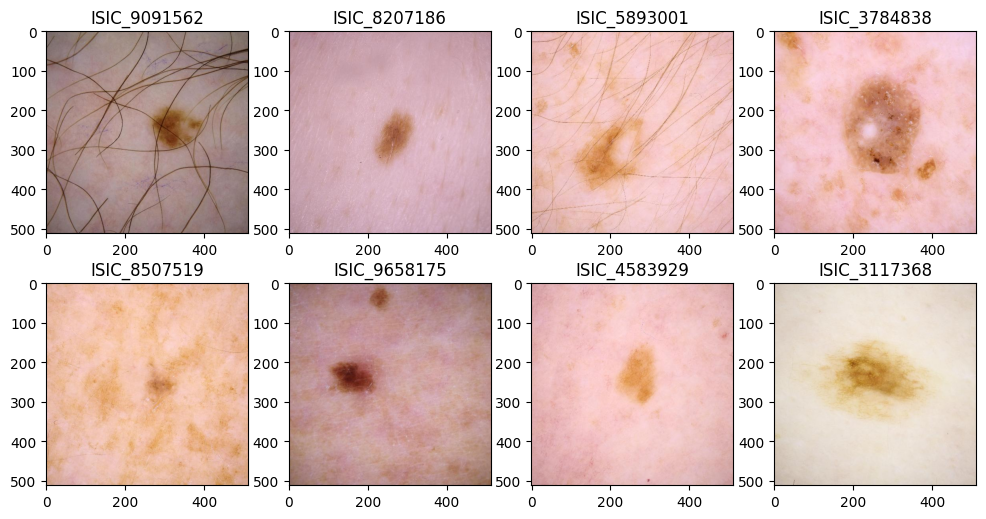
\includegraphics[width=8cm]{false_positive}
      \end{center}
      \caption{False positive examples. Often images with also little differential excitation however the histogram equalization sometimes changes the smooth excitation hill into different landscape, see Figure \ref{fig8}.}
      \label{fig5}
\end{figure}

\begin{figure}[H]
      \begin{center}
            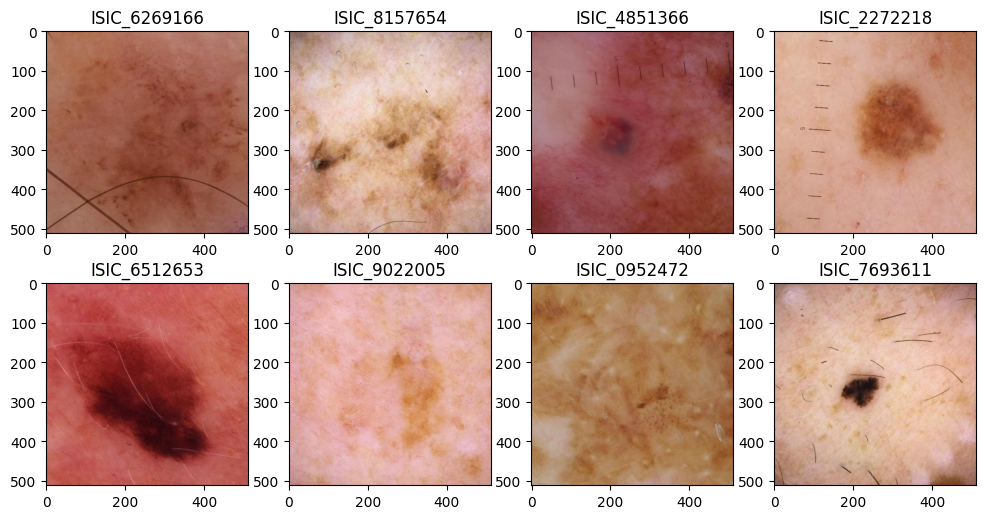
\includegraphics[width=8cm]{false_negative}
      \end{center}
      \caption{False negative samples. Usually images with melanom that looks somewhat in tolerance of normal skin.}
      \label{fig6}
\end{figure}

\begin{figure}[H]
      \begin{center}
            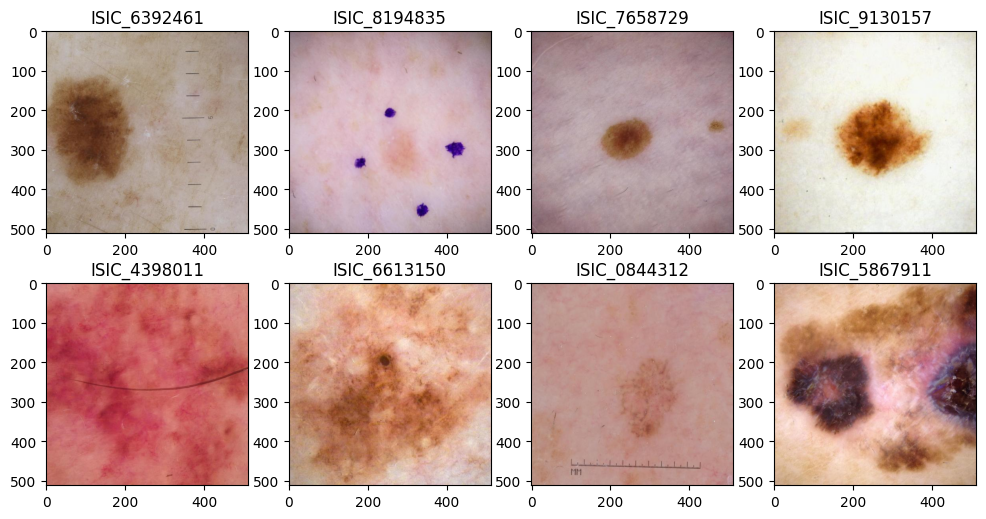
\includegraphics[width=8cm]{true_positive}
      \end{center}
      \caption{True positive samples.}
      \label{fig7}
\end{figure}

\begin{figure}[H]
       \begin{center}
              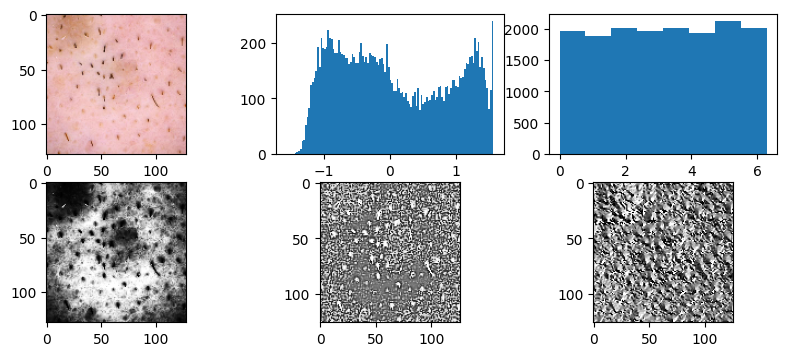
\includegraphics[width=6cm]{false_positive_overview}
              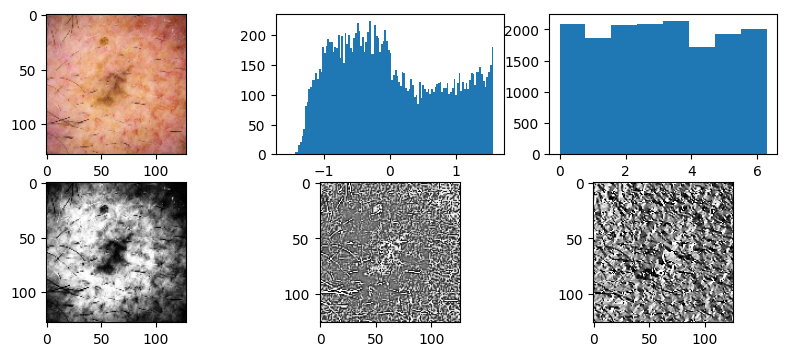
\includegraphics[width=6cm]{false_negative_overview}
       \end{center}
       \caption{Upper six is false positive (benign), lower six false negative (malignant). Pay attention the fact that in case of the benign lesion the parts with the highest differential excitation are the hairs! On the other hand the false negative WLD looks promising, however there were probably WLDs such as the false positive right above that were too close. For columns explanation see Figure \ref{fig1}.}
       \label{fig8}
\end{figure}
% 
\end{document}
